\section{Concept}

This section illustrates the concrete examples that we have come up with.

\subsection{Location Sharing}
\label{location_sharing}

todo

\subsection{Video Sharing}

todo

\subsection{Screencast Sharing}

todo

\subsection{Calendar Sharing}

todo

\subsection{Data to Go}
\label{data2go}

One part of the proposed architecture would be location aware data sharing within the display network.
This is envisioned to work in two general modes, which are based on the underlying location sharing described in section \ref{location_sharing}.
The first would allow the pinning of data to a user's location, leaving its visibility set to private.
This would allow a user to take data with him when going to a colleagues' office for a meeting.
Apart from making the data available to the system, no further care would need to be taken to keep data readily available.
The second mode would allow data to be shared by sending it to a certain location, for example a meeting room.
This would make the data publicly available, primarily for that location.

Due to the high number of personal devices that are in use in the target environment, a client program will be required for easy access to data that a user wants to share.

\begin{figure}
	\centering
	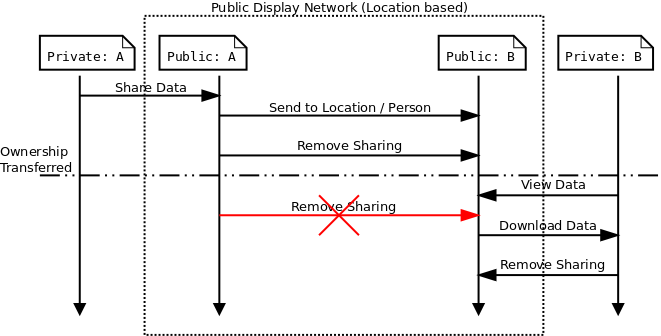
\includegraphics[width=\linewidth]{img/data_sharing.png}
	\caption[Data Sharing Sequence]{Informal sequence diagram of how data sharing might work, including some privacy and security options.}
	\label{data_share_sequence}
\end{figure}

test test
Figure \ref{data_share_sequence} shows some cool stuff, test test.
